\chapter{Background}
\label{sec:background}


\section{Boogie Language}

An excellent resource for the Boogie language is the paper by K. Rustan M. Leino \cite{leino2008boogie},
which is officially linked on the Boogie GitHub page.
\footnote{https://github.com/boogie-org/boogie}
Unfortunately, the paper is no longer entirely up-to-date with the modern development of the language.
\footnote{https://boogie-docs.readthedocs.io/en/latest/LangRef.html\#inconsistent-assumptions}\textsuperscript{,}
\footnote{https://github.com/dafny-lang/dafny/issues/4005\#issuecomment-1570363166}
Nevertheless, it remains a solid starting point, as it is the most comprehensive reference available.

\paragraph{Boogie}
This language is similar in style to Viper and Dafny, but it includes fewer high-level features.
It resembles a procedural language, featuring assignments, control-flow statements (\lstinline[columns=fixed]{if}, \lstinline[columns=fixed]{while}, \lstinline[columns=fixed]{goto}),
and side-effect-free functions and procedures, which may be polymorphic.
As an Intermediate Verification Language (IVL), it also includes \lstinline[columns=fixed]{assume}, \lstinline[columns=fixed]{assert},
and \lstinline[columns=fixed]{axiom} statements that may use quantifiers.
These constructs are used to encode specifications that define the intended correct behavior of the program.
We will not delve too deeply into the specific details of the language here,
but rather refer interested readers to the resources mentioned earlier.
The following example provides a sense of the language's syntax:


\begin{lstlisting}[caption={Example Boogie code (inspired by Dafny's encoding)}]
type Array _ _;
function lookup<Dom, Ran> (a: Array Dom Ran, i: Dom) : Ran;

type ref;
const null: ref;

type Field;

type Box;
type Heap = Array ref (Array Field Box);

function read(H: Heap, r: ref, f: Field) : Box
{
    lookup(lookup(H, r), f)
}

function assign(H: Heap, r: ref, f: Field, b: Box) : Heap;
axiom (forall heap: Heap, r: ref, f: Field, b: Box ::
  r != null ==> read(assign(heap, r, f, b), r, f) == b);

procedure positive() returns (r: int);
    free ensures r > 0;

procedure foo() returns (b: Box)
{
    var H: Heap;
    var r: ref;
    var f: Field;
    var i: int;
    var b1: Box;
    var b2: Box;

    assume r != null;
    call i := positive();

    if (i > 0)
    {
        b := b1;
    }
    else
    {
        b := b2;
    }

    H := assign(H, r, f, b);

    assert read(H, r, f) == b1;
}
\end{lstlisting}

As seen in the example, the function \lstinline[columns=fixed]{lookup} includes type parameters enclosed in \lstinline[columns=fixed]{<>},
identifying it as a polymorphic function.
Boogie allows users to declare new types using the \lstinline[columns=fixed]{type} syntax.
We will refer to values of these types as \emph{abstract values}.
Type declarations may accept type parameters,
which can be instantiated to construct new types, as demonstrated by the \lstinline[columns=fixed]{Array} example.
The \lstinline[columns=fixed]{type} keyword can also be used to create type synonyms instead of entirely new types.
Boogie allows developers to introduce global assumptions via the \lstinline[columns=fixed]{axiom} keyword.
This means the verifier assumes the property holds globally and disregards any program executions that violate the axiom.
Often, these axioms are used in conjunction with quantifiers like \lstinline[columns=fixed]{forall},
enabling the definition of properties that apply to every value of a specified type.
In the example, the procedure \lstinline[columns=fixed]{positive} is decorated with the attributes \lstinline[columns=fixed]{free ensures}.
The \lstinline[columns=fixed]{ensures} keyword specifies a post-condition of a procedure or function,
meaning the assertion must hold upon exit.
The \lstinline[columns=fixed]{free} modifier instructs Boogie to skip verifying the assertion internally,
while still allowing calling functions to assume it holds.


\section{Boogie Maps}
\label{sec:semantics-boogie-maps}

The most relevant language construct for this project is the Boogie map,
as formally supporting it forms our core contribution.
We begin by illustrating how maps can be used in Boogie:

\begin{lstlisting}[caption={Simple Boogie Map Example}]
procedure simple ()
{
    var y: int;
    var a: [int] int;
    var b: [int] int;

    y := a[0];       // select
    a := a[2 := 1];  // store and return a new map
    // convenient map assign syntax for the above
    a[2] := 1;

    // lambda expression
    a := (lambda x: int ::
      if x > 0 then y + x + x else y + x);
    b := (lambda x: int ::
      if x < 0 then y + x     else y + x + x);

    assert a == b;
}
\end{lstlisting}

Using the syntax \lstinline[columns=fixed]{var m:[D] R}, one can declare a map with domain type \lstinline[columns=fixed]{D} and range type \lstinline[columns=fixed]{R}.
With a map, developers can select a value at a given key and obtain an updated map by storing a new value at a corresponding key.
Notably, maps are total and will always return a valid return value for any key with the correct type.

Interestingly, lambda expressions can be treated as map values.
Thus, a map behaves like an extensional function that is treated as a first-class value and can be dynamically updated.
Importantly, it is \textbf{not} analogous to a dictionary or an association list in standard programming languages, as those represent strictly finite mappings.

Boogie supports more complex map types as well.
Maps can take multiple keys, referred to as multi-arity maps.
Furthermore, the domain and range types can themselves be maps, enabling nested map structures.
However, multi-arity maps are generally discouraged according to this documentation,
\footnote{https://boogie-docs.readthedocs.io/en/latest/LangRef.html\#inconsistent-assumptions}
as they can be structurally transformed into nested, single-arity maps.

\begin{lstlisting}[caption={Multi-Arity Boogie Map Example}]
procedure complex ()
{
    var y: int;
    var a: [int] int;
    var d: [ [int]int, int ] int;   // multi-arity
    var c: [ [int]int ] [int] int;  // curried

    c[a][y] := y;
    d[a, y] := y;
}
\end{lstlisting}

Maps can also be polymorphic, meaning they can accept type parameters:

\begin{lstlisting}[caption={Polymorphic Boogie Map Example}]
procedure poly ()
{
    var p: <S>[S]S;
    p[0] := 1;
    p[true] := false;
    p[p] := p;
    // impredicative polymorphism, recursive types
}
\end{lstlisting}

\footnote{Examples taken and adapted from \url{https://ethz.ch/content/dam/ethz/special-interest/infk/chair-program-method/pm/documents/Education/Courses/SS2017/Program\%20Verification/08-Boogie.pdf}.}

This is a highly powerful feature. However, fully supporting it lies outside the scope of this thesis, as outlined in our goals (Section~\ref{sec:goals-to-support}).


\section{Prior Work by Parthasarathy}
\label{sec:prior-work}

We build upon the prior work established by Parthasarathy et al.~\cite{parthasarathy2021formally}.
Proving the complete implementation of the Boogie verifier end-to-end would be a monumental task,
as it is a large, complex, and constantly evolving codebase.
Therefore, the approach taken by the prior work is to validate individual verification runs instead.
The goal is to formally prove that the validity of the outputted Verification Condition (VC)
mathematically implies the correctness of the input program.
To achieve this, we must precisely define what it means for a Boogie program to be "correct".
This requires formal semantics dictating Boogie's exact behavior.
Because such a formalization did not previously exist,
the prior work formalized a core subset of Boogie's semantics within the interactive theorem prover Isabelle/HOL.
To generate this proof, the prior work instrumented the codebase of the Boogie verifier.
This custom module produces an embedding of both the Boogie program and the VC within Isabelle/HOL.
It also gathers crucial context during translation to automatically construct the desired proof.
See Figure~\ref{fig:proofgen-pipeline} for an illustrative diagram of this architecture.

\begin{figure}[t]
  \centering
  \begin{tikzpicture}[
    >=Latex,
    font=\small,
    box/.style={draw=black, thick, minimum width=4.1cm, minimum height=0.95cm, align=center},
    sembox/.style={draw=green!55!black, thick, minimum width=4.1cm, minimum height=0.95cm, align=center},
    thinarr/.style={->, thick},
    dasharr/.style={->, thick, dashed},
    proofbox/.style={draw=orange!90!black, very thick, rounded corners=10pt, minimum width=4.2cm, minimum height=0.95cm, align=center}
  ]
    \node[box] (bp) at (0,0) {Boogie Program};
    \node[box, minimum width=1.7cm] (vc) at (9.5,0) {VC};
    \node[sembox] (sem) at (0,-2.7) {Boogie Embedding};
    \node[sembox, minimum width=1.7cm] (vcemb) at (9.5,-2.7) {VC Embedding};
    \node[proofbox] (proofgen) at (5.0,-1.15) {boogie-proofgen};
    \node[sembox, minimum width=3.8cm] (foundational) at (5.9,-4.55) {Foundational Boogie Semantics};

    \draw[thinarr, magenta!65!black] (bp.east) -- node[above, text=magenta!65!black, font=\large] {code-to-VC translation} (vc.west);
    \draw[dasharr, green!60!black] (bp.south) -- node[right, text=black] {embedding} (sem.north);
    \draw[dasharr, green!60!black] (vc.south) -- node[left, text=black] {embedding} (vcemb.north);
    \draw[thick, dashed, orange!90!black] ($(proofgen.north)+(0,0.05)$) -- ++(0,0.6);
    \draw[dasharr, orange!90!black] ($(proofgen.south)+(0,-0.05)$) -- (5.0,-2.74);
    \draw[thinarr, green!55!black] (vcemb.west) -- node[below, text=green!55!black, font=\large] {$\mathrm{valid}(VC) \models \mathrm{correct}(BP)$} (sem.east);
    \draw[thinarr, green!60!black] (foundational.north) -- node[right, text=green!55!black] {uses} (5.9,-3.3);

    \node at (-0.05,-3.55) {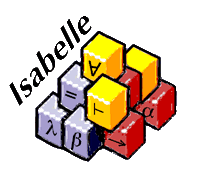
\includegraphics[width=1.15cm]{uploads/isabelle_transparent.png}};
    \node at (9.5,-3.55) {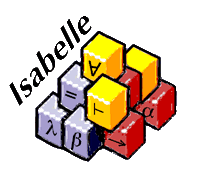
\includegraphics[width=1.15cm]{uploads/isabelle_transparent.png}};
  \end{tikzpicture}
  \caption{The Boogie verifier translates an input program into a VC.
  The proof generation module embeds both artifacts into Isabelle.
  Additionally, it generates a proof showing that the validity of the VC implies the correctness of the input program, as defined by the foundational formal semantics.
  Adapted from \cite{parthasarathy2021formally}.
  Isabelle Logo from https://isabelle.in.tum.de/logo/,
  contributed by Franziska Wenzel, Munich.}
  \label{fig:proofgen-pipeline}
\end{figure}


\section{Type Encoding \& Map Extensionality}
\label{sec:type-encoding}

Boogie provides three different ways to encode types in polymorphic programs,
as detailed by the \texttt{boogie /help} command:

\begin{lstlisting}[language=make, numbers=none,
caption={\texttt{boogie /help} output}]
/typeEncoding:<t>
  Encoding of types when generating VC of a polymorphic program:
      m = monomorphic (default)
      p = predicates
      a = arguments
  Boogie automatically detects monomorphic programs and enables
  monomorphic VC generation, thereby overriding the above option.
  If the latter two options are used, then arrays are handled via axioms.
\end{lstlisting}

Over time, the default setting has changed from predicate to monomorphic type encoding.
\footnote{https://github.com/boogie-org/boogie/pull/732}
The prior work was built when predicate type encoding was the default,
and it functions best under this configuration.
According to the documentation of the prior work,
\footnote{https://github.com/viperproject/boogie-proofgen/?tab=readme-ov-file\#supported-subset}
it does not support type declarations under other encodings,
as they fundamentally alter the structure of the resulting VC.

To force predicate type encoding, one must use the flag \texttt{/typeEncoding:p}
and ensure polymorphic code exists in the input.
If no such code exists naturally, one can inject a dummy function
(e.g., \lstinline[columns=fixed]{function dummy<T>(x: T) : T;}).
Otherwise, the Boogie verifier will override the command-line option and forcefully monomorphize the types.

The chosen type encoding also profoundly impacts the VC representation of maps,
even if those maps are monomorphic.
A key difference is that the monomorphic type encoding allows maps to be modeled directly via SMT arrays.
Because SMT arrays are inherently extensional, it follows that under this encoding, Boogie maps are extensional as well.
\footnote{This contradicts an outdated assertion in the paper "This is Boogie 2" \cite{leino2008boogie}, which claims maps are not guaranteed to be extensional.}
Extensionality implies that two maps are considered equal if they behave identically,
meaning if for all keys in their domain, the select operation yields the same return value.


\section{Boogie Map VC Predicate Encodings}
\label{sec:vc-axioms-changes}
\label{sec:vc-map-axioms}
\label{sec:vc-structure}

% TODO cite correctly
Let us examine the overall structure of the Isabelle embedding of the generated VC
(adapted from the prior work \cite{parthasarathy2021formally}):


\[
\forall
\underbrace{\textit{VC quantifiers}}_{\substack{
  \text{type encoding parameters,}\\
  \text{functions, variable values}\\
  \textbf{map types \& functions}}}
\mathpunct{.}\;
\Bigl(
\underbrace{\textit{VC assumptions}}_{\substack{
  \text{type encoding,}\\
  \text{fun./var./prog. axioms}\\
  \textbf{map axioms}}}
\Longrightarrow
\textit{WP}
\Bigr)
\]


This structure forms a logical implication:
a model fulfilling a specific set of assumptions implies a Weakest Precondition (WP).
This weakest precondition is essential for demonstrating the correctness of the input program.
Therefore, our formal semantic modeling of Boogie must rigorously satisfy these assumptions,
providing clear formal targets that the semantics must achieve.
Supporting maps introduces additional functions and axioms to the VC,
governing map types and behaviors.
These axioms differ significantly depending on the type encoding used.
Since the prior work relies on predicate type encoding,
we focus strictly on its specific encoding of maps.
The following represents the map-relevant portions of the VC.


\providecommand{\MapType}{\operatorname{MapType}}
\providecommand{\MapTypeInvK}{\operatorname{MapTypeInv0}}
\providecommand{\MapTypeInvV}{\operatorname{MapTypeInv1}}
\providecommand{\Select}{\operatorname{MapSelect}}
\providecommand{\Store}{\operatorname{MapStore}}
\providecommand{\type}{\operatorname{type}}


There are the sorts $U$ and $T$, where $U$ represents values, $T$ represents types,
and a function $\type : U \rightarrow T$ that determines the type of a given value.
Additionally, the following functions are introduced:
\footnote{We have simplified the axioms slightly for clarity.}
\begin{itemize}
  \item $\Select : (U, U) \rightarrow U$, selecting a value from a map.
  \item $\Store : (U, U, U) \rightarrow U$, updating a map.
  \item $\MapType : (T, T) \rightarrow T$, constructing a map type from two component types.
  \item $\MapTypeInvK : T \rightarrow T$, extracting the domain type.
  \item $\MapTypeInvV : T \rightarrow T$, extracting the range type.
\end{itemize}

Notably, these functions technically apply to \emph{all} values in the logic, not just map values.
They must satisfy the following axioms:

\begin{align*}
  & \forall\ k\ v.\ \MapTypeInvK\ (\MapType\ k\ v) = k\\
  & \forall\ k\ v.\ \MapTypeInvV\ (\MapType\ k\ v) = v
\end{align*}

These axioms guarantee that $\MapTypeInvK$ and $\MapTypeInvV$ act as true inverse functions of the map type constructor $\MapType$.

\begin{equation}
  \label{ax:map-select-typesafe}
  \begin{aligned}
    \forall \ m \ k. \
    \type \ m = \MapType \ (\type \ k) \ (\MapTypeInvV \ (\type \ m)) \\
    \implies  \type \ (\Select \ m \ k) = \MapTypeInvV \ (\type \ m)
  \end{aligned}
\end{equation}

This enforces type safety: if we select from a map using a key of the correct domain type,
the result is guaranteed to be of the corresponding range type.

\begin{align*}
  &\forall \ m \ k \ v. \\
  &\type m = \MapType\ (\type\ k)\ (\type\ v) \\
  &\implies  \type(\Store\ m\ k\ v) = \MapType\ (\type\ k)\ (\type\ v)
\end{align*}

This dictates that the store operation returns a new map of the identical type.

\begin{equation}
  \label{ax:map-update-strong}
  \begin{aligned}
    &\forall \ m \ k \ v.\\
    &\type\ v = \MapTypeInvV\ (\type\ m) \\
    &\implies  \Select\ (\Store\ m\ k\ v)\ k = v
  \end{aligned}
\end{equation}

This confirms that the store operation successfully updates the value at a specific position.

\begin{align*}
  &\forall \ m \ x \ y \ v.\\
  &x = y \ \vee \\
  &\Select\ (\Store\ m\ x\ v)\ y = \Select\ m\ y
\end{align*}

This stability axiom demonstrates that storing a value at one position
does not inadvertently alter the values at other positions.


\section{SMT and SMT-LIB}
SMT stands for Satisfiability Modulo Theories \cite{barrett2010smt}.
It is a decision problem used to determine whether a mathematical formula is satisfiable under practical background theories,
which help model common structures such as arrays or real numbers.
This format is used to encode the VC output of the Boogie verifier.

The language is standardized as SMT-LIB.
Extensive documentation can be found in "The SMT-LIB Standard" paper~\cite{barrett2010smt},
and various online resources provide comprehensive tutorials on writing and evaluating SMT queries.
\footnote{https://www.philipzucker.com/z3-rise4fun/guide.html}\textsuperscript{,}
\footnote{https://microsoft.github.io/z3guide/docs/theories/Arrays/}\textsuperscript{,}
\footnote{https://theory.stanford.edu/\~nikolaj/programmingz3.html}


\section{Interactive Theorem Provers (ITPs)}

The proof generation module produces its certificates in the proof language of Isabelle/HOL.
Isabelle/HOL is an Interactive Theorem Prover (ITP).
Other prominent ITPs include Rocq\footnote{https://rocq-prover.org/}
\cite{huet1997coq}
and Lean\footnote{https://lean-lang.org/} \cite{de2015lean}.
These systems assist in the mechanical construction of mathematical proofs on a computer
and rigidly verify that the mechanized proofs are logically sound.

\subsection{Isabelle/HOL}
\label{sec:isabelle}
In contrast to many other ITPs, Isabelle/HOL is not based on dependent type theory.
Isabelle itself serves as a generic meta-framework used to build specific logical systems.
Isabelle/HOL is one such implementation, where HOL stands for Higher-Order Logic.
It operates by combining functional programming (using Haskell-style syntax) with formal logic.
We refer the reader to the extensive official tutorial \cite{nipkow2002isabelle}
and the project website\footnote{https://isabelle.in.tum.de/} for deeper information.
Here, we briefly introduce a few advanced features used heavily throughout this project:

\paragraph{Sum Types}\footnote{https://isabelle.in.tum.de/library/HOL/HOL/Sum\_Type.html}
We can combine two existing types to create a union type.
For example, \isa{int + bool} represents a type that can be either an integer \emph{or} a boolean.
Both constituent types provide their own datatype constructors:
\isa{Inl} injects a value into the left type,
and \isa{Inr} injects a value into the right type.
Therefore, both \isa{Inl 42 :: (int + bool)} and \isa{Inr True :: (int + bool)} represent valid instances of this sum type.

\paragraph{Inductive Definitions}\footnote{Chapter 7 in \cite{nipkow2002isabelle}}
Inductive definitions define predicates by describing only the positive cases.
They allow us to mark a property as true by building recursively upon previously established truths.
This is particularly useful when negative cases are difficult to describe directly.

Consider defining a property that describes whether a number eventually reaches one according to the Collatz conjecture rules:

\begin{isabellebody} \isanewline
\isakeywordONE{fun}\isamarkupfalse%
\ ends{\kern0pt}\ \isakeywordTWO{where}\isanewline
\ \ {\isachardoublequoteopen}ends{\kern0pt}\ {\isadigit{1}}{\kern0pt}\ {\isacharequal}{\kern0pt}\ True{\isachardoublequoteclose}\ {\isacharbar}{\kern0pt}\isanewline
\ \ {\isachardoublequoteopen}ends{\kern0pt}\ n\ {\isacharequal}{\kern0pt}\ {\isacharparenleft}{\kern0pt}if\ {\isacharparenleft}{\kern0pt}even\ n{\isacharparenright}{\kern0pt}\ then\ ends{\isacharparenleft}{\kern0pt}n\ div\ {\isadigit{2}}{\isacharparenright}{\kern0pt}\ else\ ends{\isacharparenleft}{\kern0pt}{\isadigit{3}}{\isacharasterisk}{\kern0pt}n\ {\isacharplus}{\kern0pt}\ {\isadigit{1}}{\isacharparenright}{\kern0pt}{\isacharparenright}{\kern0pt}{\isachardoublequoteclose}\isanewline
%
\ \ \ \isamarkupcmt{invalid definition: Could not find lexicographic termination order.}\isanewline
\end{isabellebody}


Such a direct function definition is rejected by Isabelle, as we cannot guarantee termination upfront.
Instead, using an inductive definition, we can build the positive cases structurally from the ground up:

\begin{isabellebody} \isanewline
\isakeywordONE{inductive}\isamarkupfalse%
\ ends\ \isakeywordTWO{where}\isanewline
\ \ base{\isacharcolon}{\kern0pt}\ {\isachardoublequoteopen}ends\ {\isadigit{1}}{\isachardoublequoteclose}\ {\isacharbar}{\kern0pt}\isanewline
\ \ two{\isacharcolon}{\kern0pt}\ {\isachardoublequoteopen}ends\ n\ {\isacharequal}{\kern0pt}{\isacharequal}{\kern0pt}{\isachargreater}{\kern0pt}\ ends\ {\isacharparenleft}{\kern0pt}{\isadigit{2}}{\isacharasterisk}{\kern0pt}n{\isacharparenright}{\kern0pt}{\isachardoublequoteclose}\ {\isacharbar}{\kern0pt}\isanewline
\ \ three{\isacharcolon}{\kern0pt}\ {\isachardoublequoteopen}ends\ {\isacharparenleft}{\kern0pt}{\isadigit{3}}{\isacharasterisk}{\kern0pt}n{\isacharplus}{\kern0pt}{\isadigit{1}}{\isacharparenright}{\kern0pt}\ {\isacharequal}{\kern0pt}{\isacharequal}{\kern0pt}{\isachargreater}{\kern0pt}\ ends\ n{\isachardoublequoteclose}\isanewline
\end{isabellebody}

As demonstrated, we can recurse smoothly within inductive definitions.
However, not all structures are admissible.
Crucially, recursion may not appear in a negative position:

\begin{isabellebody} \isanewline
\isakeywordONE{inductive}\isamarkupfalse%
\ even\ \isakeywordTWO{where}\isanewline
\ \ base{\isacharcolon}{\kern0pt}\ {\isachardoublequoteopen}even\ {\isadigit{0}}{\isachardoublequoteclose}\ {\isacharbar}{\kern0pt}\isanewline
\ \ step{\isacharcolon}{\kern0pt}\ {\isachardoublequoteopen}{\isasymnot}even\ n\ {\isacharequal}{\kern0pt}{\isacharequal}{\kern0pt}{\isachargreater}{\kern0pt}\ even\ {\isacharparenleft}{\kern0pt}Suc\ n{\isacharparenright}{\kern0pt}{\isachardoublequoteclose}\isanewline
%
\ \ \isamarkupcmt{invalid definition: monotonicity proof failed}
\end{isabellebody}

Such a structure is prohibited because an inductive definition cannot reason about negative cases
while the property itself is still actively being defined.

\paragraph{Locales}\footnote{https://isabelle.in.tum.de/doc/locales.pdf}
We can isolate environments by setting up locales in Isabelle/HOL:

\begin{isabellebody} \isanewline
\isakeywordONE{locale}\isamarkupfalse%
\ foo\ {\isacharequal}{\kern0pt}\isanewline
\ \ \isakeywordTWO{fixes}\ f\ {\isacharcolon}{\kern0pt}{\isacharcolon}{\kern0pt}\ {\isachardoublequoteopen}nat\ {\isacharequal}{\kern0pt}{\isachargreater}{\kern0pt}\ nat{\isachardoublequoteclose}\isanewline
\ \ \isakeywordTWO{fixes}\ x\ {\isacharcolon}{\kern0pt}{\isacharcolon}{\kern0pt}\ nat\isanewline
\ \ \isakeywordTWO{assumes}\ {\isachardoublequoteopen}f\ x\ {\isacharequal}{\kern0pt}\ x{\isachardoublequoteclose}\isanewline
%
\isakeywordTWO{begin}\isanewline
%
\ \isamarkupcmt{Context-specific definitions and proofs%
}\isanewline
\isakeywordTWO{end}\isamarkupfalse%
\end{isabellebody}


Inside this locale, we can refer directly to the fixed constants and make assumptions about them.
If we wish to extend the locale to other theory files, we use the \isakeywordONE{context} command:

\begin{isabellebody}\isanewline
\isakeywordONE{context}\isamarkupfalse%
\ foo\isanewline
\isakeywordTWO{begin}\isanewline
%
\ \isamarkupcmt{Locale Extensions}\isanewline
\isakeywordTWO{end}\isamarkupfalse%
\end{isabellebody}

To apply the definitions and proofs from the locale to concrete values, we instantiate them:

\begin{isabellebody}\isanewline
\isakeywordONE{interpretation}\isamarkupfalse%
\ foo\ g\ {\isadigit{3}}\isanewline
\ \ %
\isamarkupcmt{proof showing that g 3 = 3}\isanewline
\end{isabellebody}

In this case, we instantiate \isa{f} with \isa{g} and \isa{x} with \isa{3}, discharging the proof obligation that \isa{f x = x}.
Following the interpretation, all definitions become available globally with the instantiated values.
Crucially, a locale can only be interpreted once within a given theory path.
Therefore, one must ensure all necessary theories are imported prior to interpretation.
Otherwise, their contexts will remain uninstantiated.

\paragraph{Type Definitions from Sets}\footnote{Section 8.5.2 in \cite{nipkow2002isabelle}}
As previously noted, Isabelle/HOL does not support dependent types.
However, we can still construct restricted types based on existing values by converting non-empty sets into types.
In fact, types in Isabelle/HOL are formally interpreted as non-empty sets \cite{kunvcar2016types}.

\begin{isabellebody}\isanewline
\isakeywordONE{typedef}\isamarkupfalse%
\ t\ {\isacharequal}{\kern0pt}\ {\isachardoublequoteopen}{\isacharbraceleft}{\kern0pt}{\isadigit{0}}{\isacharcolon}{\kern0pt}{\isacharcolon}{\kern0pt}nat{\isacharcomma}{\kern0pt}\ {\isadigit{1}}{\isacharcomma}{\kern0pt}\ {\isadigit{4}}{\isadigit{2}}{\isacharcomma}{\kern0pt}\ {\isadigit{6}}{\isadigit{7}}{\isacharbraceright}{\kern0pt}{\isachardoublequoteclose}%
\ \isakeywordONE{by}\isamarkupfalse%
\ auto%
\end{isabellebody}

We only need to prove that the defining set is not empty.

The reason it that all Isabelle/HOL types are defined to be non-empty.
This type definition is even permitted to depend on a type parameter by providing the \isa{overloaded} keyword:

\begin{isabellebody}\isanewline
\isakeywordONE{abbreviation}\isamarkupfalse%
\ p\ {\isacharcolon}{\kern0pt}{\isacharcolon}{\kern0pt}\ {\isachardoublequoteopen}{\isacharparenleft}{\kern0pt}{\isacharprime}{\kern0pt}a\ list{\isacharparenright}{\kern0pt}\ set{\isachardoublequoteclose}\ \isakeywordTWO{where}\isanewline
\ \ {\isachardoublequoteopen}p\ {\isasymequiv}\ {\isacharbraceleft}{\kern0pt}l{\isachardot}{\kern0pt}\ {\isasymnot}\ {\isacharparenleft}{\kern0pt}l\ {\isacharequal}{\kern0pt}\ {\isacharbrackleft}{\kern0pt}{\isacharbrackright}{\kern0pt}{\isacharparenright}{\kern0pt}{\isacharbraceright}{\kern0pt}{\isachardoublequoteclose}\isanewline
\isanewline
\isakeywordONE{typedef}\isamarkupfalse%
\ {\isacharparenleft}{\kern0pt}\isakeywordTWO{overloaded}{\isacharparenright}{\kern0pt}\ {\isacharprime}{\kern0pt}a\ tp\ \ {\isacharequal}{\kern0pt}\ {\isachardoublequoteopen}p\ {\isacharcolon}{\kern0pt}{\isacharcolon}{\kern0pt}\ {\isacharparenleft}{\kern0pt}{\isacharprime}{\kern0pt}a\ list{\isacharparenright}{\kern0pt}\ set{\isachardoublequoteclose}%
\ \isakeywordONE{by}\isamarkupfalse%
\ auto%
\end{isabellebody}

A notable limitation of this feature is that \isa{typedef} commands cannot be used inside a locale context.
\footnote{Though workarounds may be possible, see \cite{kunvcar2016types}.}

\paragraph{Type Classes}\footnote{https://isabelle.in.tum.de/doc/classes.pdf}
Isabelle allows developers to assign Haskell-style type classes to type parameters.
This guarantees that specific functions or properties are available when instantiating the type,
operating similarly to interfaces in standard programming languages.

\begin{isabellebody}\isanewline
\isakeywordONE{class}\isamarkupfalse%
\ c\ {\isacharequal}{\kern0pt}\isanewline
\ \ \isakeywordTWO{fixes}\ tonat\ {\isacharcolon}{\kern0pt}{\isacharcolon}{\kern0pt}\ {\isachardoublequoteopen}{\isacharprime}{\kern0pt}a\ {\isasymRightarrow}\ nat{\isachardoublequoteclose}\isanewline
\isanewline
\isakeywordONE{datatype}\isamarkupfalse%
\ {\isacharprime}{\kern0pt}a{\isacharcolon}{\kern0pt}{\isacharcolon}{\kern0pt}c\ D\ {\isacharequal}{\kern0pt}\ Con\ {\isacharprime}{\kern0pt}a\isanewline
\isanewline
\isakeywordONE{instantiation}\isamarkupfalse%
\ bool\ {\isacharcolon}{\kern0pt}{\isacharcolon}{\kern0pt}\ c\ \isakeywordTWO{begin}\isanewline
\ \ \isakeywordONE{fun}\isamarkupfalse%
\ c{\isacharunderscore}{\kern0pt}bool\ \isakeywordTWO{where}\ {\isachardoublequoteopen}c{\isacharunderscore}{\kern0pt}bool\ True\ {\isacharequal}{\kern0pt}\ {\isadigit{1}}{\isachardoublequoteclose}\ {\isacharbar}{\kern0pt}\ {\isachardoublequoteopen}c{\isacharunderscore}{\kern0pt}bool\ False\ {\isacharequal}{\kern0pt}\ {\isadigit{0}}{\isachardoublequoteclose}\isanewline
\ \ \isakeywordONE{instance}\isamarkupfalse%
%
% \isadelimproof
% \ %
% \endisadelimproof
%
% \isatagproof
\ \isakeywordONE{{\isachardot}{\kern0pt}{\isachardot}{\kern0pt}}\isamarkupfalse%
% %
% \endisatagproof
% {\isafoldproof}%
% %
% \isadelimproof
% %
% \endisadelimproof
\ \isanewline
\isakeywordTWO{end}\isamarkupfalse%
\isanewline
\isanewline
\isakeywordONE{term}\isamarkupfalse%
\ {\isachardoublequoteopen}Con\ False\ {\isacharcolon}{\kern0pt}{\isacharcolon}{\kern0pt}\ bool\ D{\isachardoublequoteclose}\isanewline
\end{isabellebody}

While locales are generally more flexible (accommodating multiple type parameters and arbitrary values),
type classes offer a crucial advantage for our architecture:
a \isakeywordTWO{typedef} can directly leverage a type class constraint in its definition.
This allows us to construct robust, globally constrained types predicated upon existing inductive properties.
